\chapter{Results}\label{chap:results}
The designed system has been tested in order to check the fulfillment of the functional requirements stated in \autoref{sec:requirements}. The results include both simulations of the full system and plots obtained after performing real tests with the vessel.

\section{Controller Requirements}
\begin{itemize}
  \item[\textbf{A:}] It shall be possible to select the area in which the bathymetric measurements are to be performed.
  \item[\textbf{B:}] The ASV shall be able to plan a route, such that the entire survey area is mapped.
  \item[\textbf{C:}] The ASV shall be able to follow the planned route.
  \item[\textbf{D:}] The controller shall be robust to external disturbances.
\end{itemize}

The area to survey is selected by giving the four corner points. Then, the path generation algorithm selects the needed waypoints to cover it, depending on the beamwidth.

Once these waypoints are selected, the outer controller sets the appropriate references for both speed, $\dot{x}_\mathrm{b}$, and heading, $\psi$, to the inner controller. The performance of the outer controller when using both inner controllers can be seen in \autoref{sec:pathSim}. The figures are included here as well, in order to check the fulfillment of the requirements.

\autoref{fig:path_lqr} shows the simulation results of the path followed by the vessel in the survey area when using the LQR as inner controller. The results are also shown in \autoref{fig:distlqr2} by plotting the error to the reference path.
\begin{figure}[H]
    \captionbox  
    {            
        Performance of the path following algorithm using the LQR as inner controller. The system is experiencing wind, current and wave disturbances, model perturbations and measurement noise.
        \label{fig:path_lqr}                               
    }                                                                
    {                                                                 
        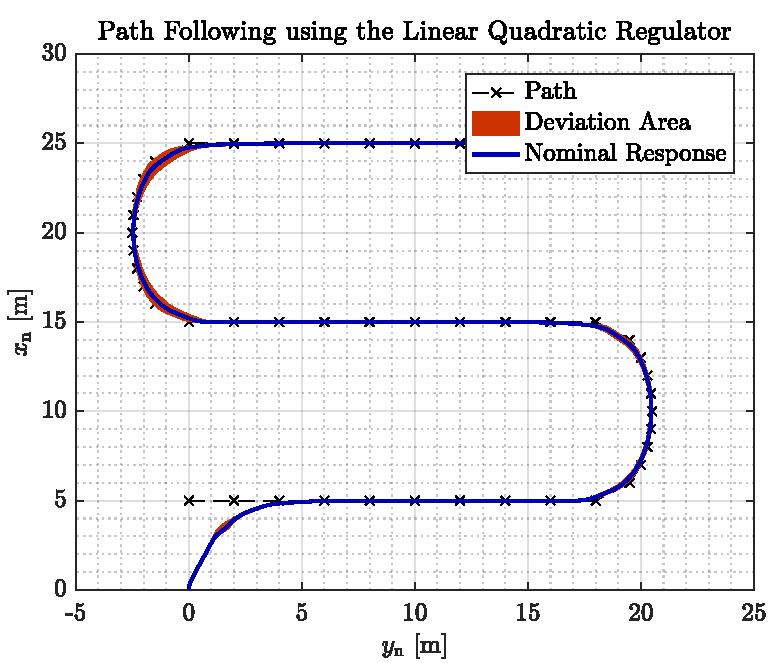
\includegraphics[width=.45\textwidth]{figures/path_lqr}    
    }                                                                  
    \hspace{5pt}                                                        
    \captionbox 
    {       
        Distance to the path when using the following algorithm and the LQR inner controller.                                                                  %\                         %\
        \label{fig:distlqr2}                                  
    }                                                                          
    {                                                                            
        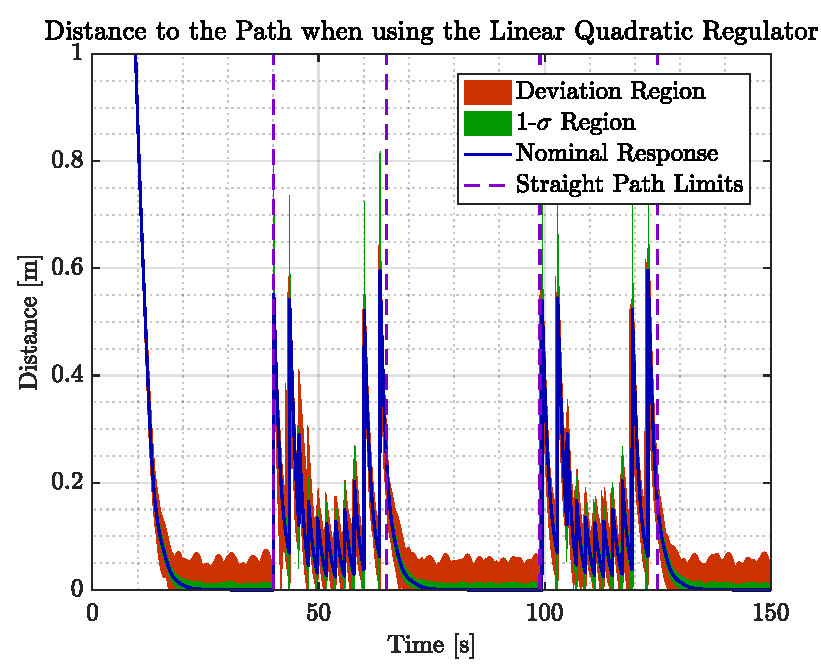
\includegraphics[width=.45\textwidth]{figures/dist_lqr}          
    }                                                                            
\end{figure}
It can be seen that the distance to the path is kept below 10 cm in the straight parts of the path, which correspond to the given area, while the distance in the curved sections is not relevant for the survey task. This accuracy is deemed sufficient for the control system of a survey vessel as the tracking accuracy is not critical for this type of application.

The path has also been tracked using the $\mathcal{H}_\infty$ inner controller as seen in \autoref{fig:path_rob2} and \ref{fig:dist_rob2}.
\begin{figure}[H]
    \captionbox 
    {   
        Performance of the path following algorithm using the $\mathcal{H}_\infty$ as inner controller. The system is experiencing wind, current and wave disturbances, model perturbations and measurement noise. \label{fig:path_rob2}
    }                                                                 
    {                                                                  
        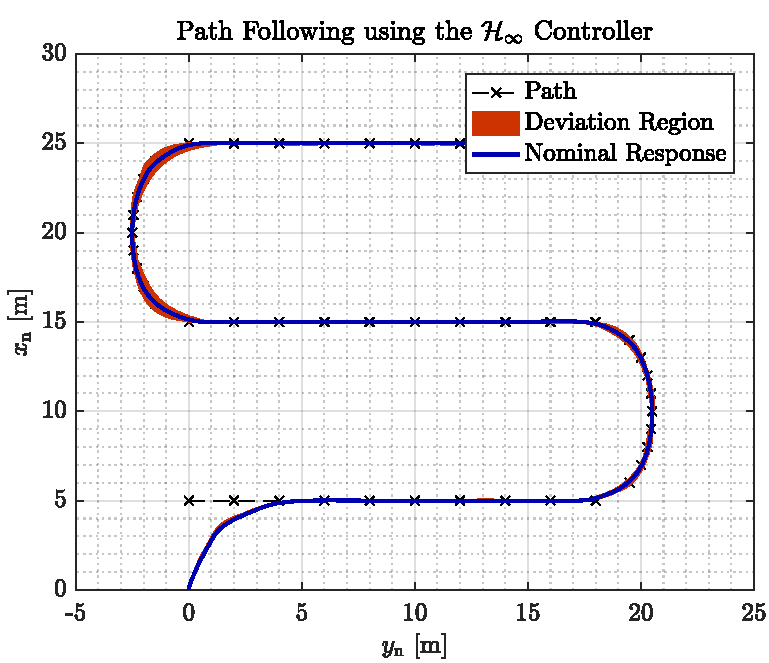
\includegraphics[width=.45\textwidth]{figures/path_rob}         
    }                                                                    
    \hspace{5pt}                                                          
    \captionbox  
    {      
        Distance to the path when using the algorithm based on $\psi_\mathrm{ref}=\chi-\beta$ and the $\mathcal{H}_\infty$ inner controller. \label{fig:dist_rob2}
    }                                                                          
    {
        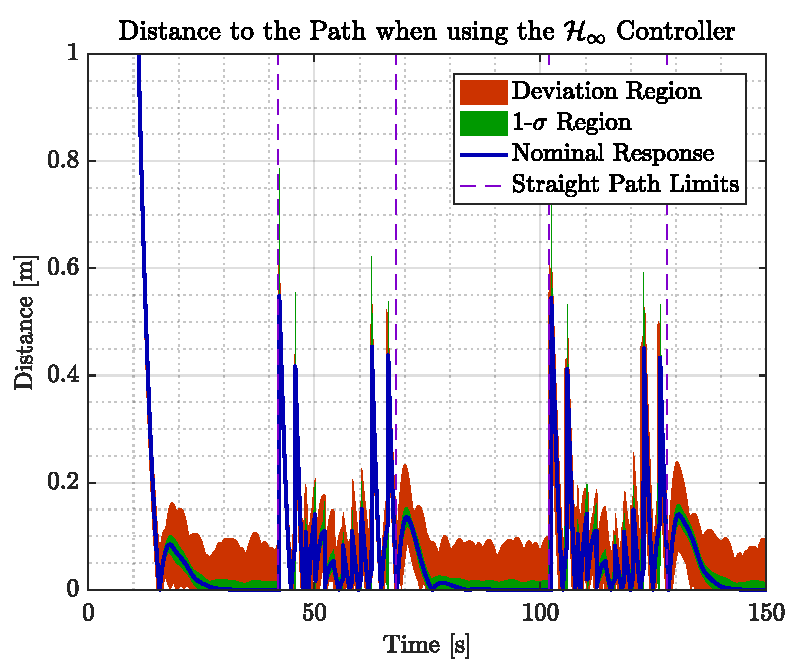
\includegraphics[width=.45\textwidth]{figures/dist_rob}
    }
\end{figure}
In this case, the path is also adequately tracked as the maximum deviation in the straight line segments is approximately 15 cm, staying below 10 cm for most of the survey path segments.

According to the results of the simulations, it can be said that the vessel follows the path through the waypoints when they are part of a straight line section of the path. In curved sections, the vessel joins smoothly the straight line segments that approximate the curve. 

Since the simulation includes disturbances, noise and parameter variation, the robustness of the controller against them has also been tested. In many cases, and especially for bathymetric measurements, the algorithm can be considered suitable.


\section{Implementation Requirements}
\begin{itemize}
  \item[\textbf{E:}] The THU shall not exceed 30 cm with a 95\% confidence interval.
  \item[\textbf{F:}] The ASV shall record and store data locally for extraction at the end of the survey.
  \item[\textbf{G:}] It shall be possible to give the ASV a command to stop and steer it back to land.
\end{itemize}

As it can be seen in \fxnote{GPS test appendix} the position measurements of the GPS are done with.....

The implementation in ROS allows to record all the topics, which contain all the sensor, estimation and inputs needed, in order to process and analyze the data afterwards.

A VPN has been set up such that it is possible to connect to the vessel remotely, allowing to run and stop the nodes when needed. A node for manual control has been added as well, such that it is possible to remotely move and control the vessel

Using the ROS implementation the controllers designed for the ASV were tested. This has been done as explained in \autoref{app:Inner}. It was seen that the designed LQR and $\mathcal{H}_\infty$ controllers were too aggressive and were not able to sufficiently stabilize the vessel. This led to a redesign of the LQR controller such that the weight matrices $\vec{Q}$ and $\vec{R}$ have been tuned such that the maximum force has been reduced while the maximum allowable value for the states has been increased to reduce the aggressiveness of the controller.
  
%The new $\vec{Q}$ and $\vec{R}$ matrices are 
%\begin{flalign}
%	\vec{Q} &= diag\left(\frac{1}{1}, 0, 0, 0, 0, 0, 0\right)\ , \nonumber \\
%	\vec{R} &= diag\left(0, 0, 0, 0\right)\ . 
%\end{flalign}
%
%\begin{flalign}
%    \vec{Q} = 
%    \begin{bmatrix}
%        100 & 0   & 0   & 0   & 0   & 0 \\
%        0   & 100 & 0   & 0   & 0   & 0 \\
%        0   & 0   & 100 & 0   & 0   & 0 \\
%        0   & 0   & 0   & 100 & 0   & 0 \\
%        0   & 0   & 0   & 0   & 4   & 0 \\
%        0   & 0   & 0   & 0   & 0   & 4
%    \end{bmatrix},
%    \rule{30px}{0px}
%    \vec{R} =
%    \begin{bmatrix}
%        2.5\times10^-3 	& 0   \\
%        0   			& 2.5\times10^-3 
%    \end{bmatrix} \ .
%\end{flalign}
%%
With these new weight matrices, a new controller was calculated such that the controller gains are
%
\begin{flalign}
    \vec{F} = 
    \begin{bmatrix}
        124.3988  &	113.7050   &	88.7435 \\
        -124.3988 &	-113.7050  &	88.7435
    \end{bmatrix},
    \rule{30px}{0px}
    \vec{F}_\mathrm{I} =
    \begin{bmatrix}
        -20.6709 & 	-17.7744	\\
        20.6709  &	-17.7744
    \end{bmatrix} \ .
\end{flalign}
%
It should also be noted that the Kalman filter for the position gave inaccurate measurements for the speed, $\dot{x}_\mathrm{b}$. Due to this and time constraints that made it infeasible to solve the problem, the Kalman filter implementation from \cite{thesis} was used to obtain a reliable $\dot{x}_\mathrm{b}$.

This new controller has been tested by tracking a reference in heading while keeping a constant speed. The results can be seen in \autoref{fig:inner_yaw} and \ref{fig:inner_xbdot}.
%
\begin{figure}[H]
    \captionbox 
    {   
        Step response in $\psi$ with a reference of -1 rad.
        \label{fig:inner_yaw}
    }                                                                 
    {                                                                  
        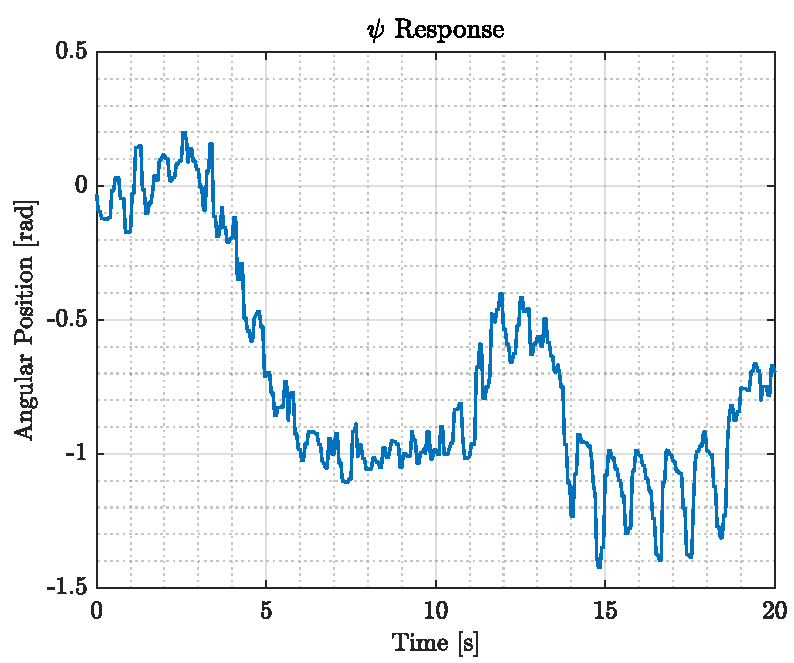
\includegraphics[width=.45\textwidth]{figures/inner_yaw}         
    }                                                                    
    \hspace{5pt}                                                          
    \captionbox  
    {      
        Step response in $\dot{x}_\mathrm{b}$ with a reference of 1 m$\cdot$s$^{-1}$.
        \label{fig:inner_xbdot}
    }                                                                          
    {
        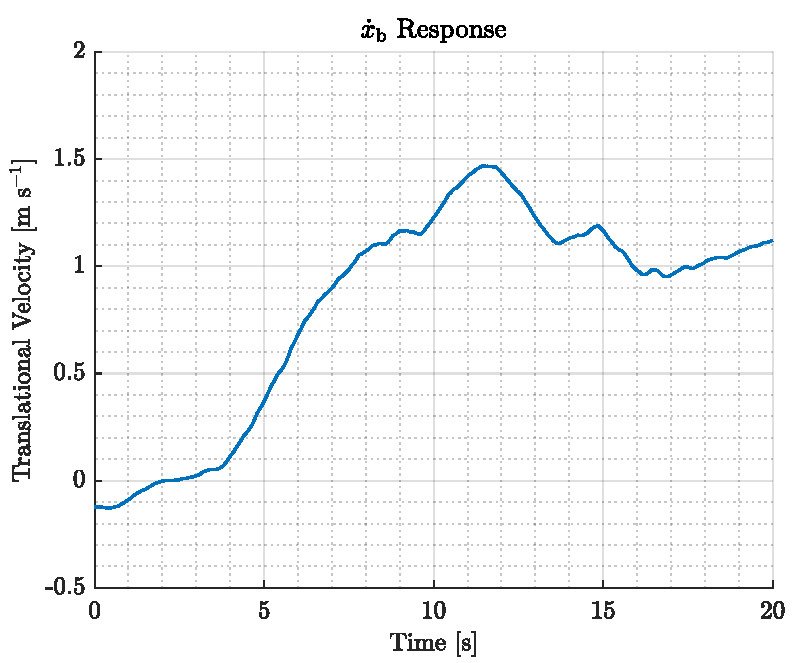
\includegraphics[width=.45\textwidth]{figures/inner_xbdot}
    }
\end{figure}

The response in $\psi$ shows that the controller is able to track a reference, specially in the first five seconds. Afterwards, the boat is disturbed, at approximately 11 s, and the yaw angle deviates from its references. Once the perturbation is compensated by the controller, the reference is tracked again. It is worth mentioning the oscillations seen from 14 to 19 seconds. They are likely due to errors when estimating $\psi$ in the Kalman filter. This can be deduced as the vessel dynamics do not allow an oscillation of 0.4 rad of approximately 1 Hz. With high probability, these oscillations are lower in the real behavior of the vessel and have been, for this particular period, amplified by the Kalman filter.

The $\dot{x}_\mathrm{b}$ response also shows a controller capable of tracking the reference. In this case, there is an overshoot in the speed response, it goes to approximately 1.2 m$\cdot$s$^{-1}$. It is important to disregard the deviation seen from 10 to 13 seconds as this corresponds to a perturbation suffered by the vessel while the test was running. After the controller recovers control of the speed, it can be seen that the speed converges to the desired reference of 1 m$\cdot$s$^{-1}$. 

Due to time constraints, the performance of the outer controller could not be tested with success in the real vessel, but the implementation done in ROS suggests a working outer controller as shown in \autoref{app:ModelNode}. In this appendix the code implemented is tested in order to check if it is working together as expected. The result is also shown in \autoref{fig:model_node_path2}.
\begin{figure}[H]
    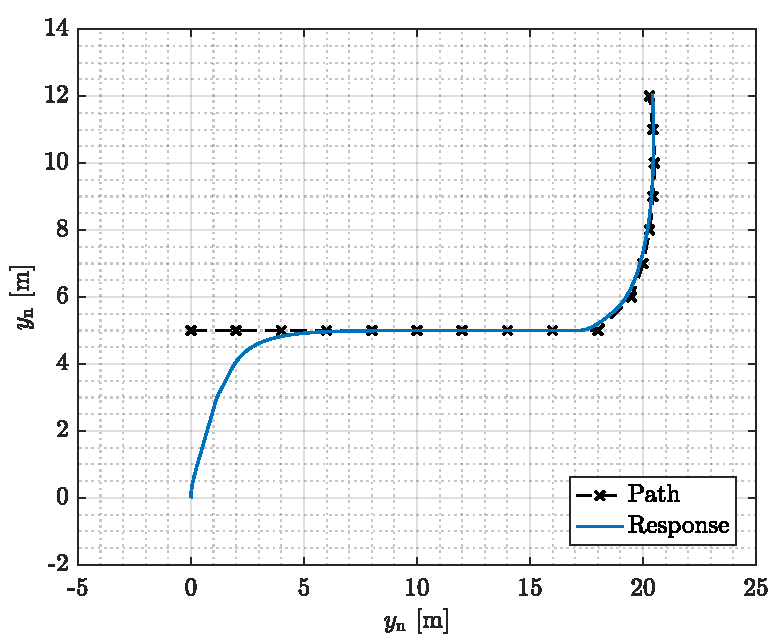
\includegraphics[width=.45\textwidth]{figures/model_node_path}
    \caption{Path and response of the implemented code, both the inner and the outer controllers together with the model node.}
    \label{fig:model_node_path2}
\end{figure}